\documentclass[spanish]{beamer}
\usepackage[ansinew]{inputenc} % Acepta caracteres en castellano
\usepackage[spanish]{babel}    % silabea palabras castellanas
\usepackage{amsmath}
\usepackage{mathtools,cancel} % cancela con una flecha \cancelto{0}{XXXX}
\renewcommand{\CancelColor}{\color{red}} %change cancel color to red
\usepackage{amsfonts}
\usepackage{braket}
\usepackage{amssymb}
\usepackage{dsfont}
\usepackage{graphicx}
\usepackage{geometry}
\usetheme{Madrid}
\usecolortheme{beaver}
\usepackage{textpos}
% Logo  en el comienzo 
\addtobeamertemplate{frametitle}{}{%
\begin{textblock*}{100mm}(.85\textwidth,-1cm)
{\includegraphics[height=0.4in, keepaspectratio=true]{/Users/luisnunez/Dropbox/MisDocumentos/UIS/UISImagenInstitucional/UISLOGO.png}}
\end{textblock*}}

\begin{document}

\title{\textbf{Computaci�n Cu�ntica} }
\author[L.A. N��ez]{\textbf{Luis A. N��ez}}  
\institute[UIS]{\textit{Escuela de F�sica, Facultad de Ciencias, } \\
\textit{Universidad Industrial de Santander, Santander, Colombia } \\
{\includegraphics[height=0.4in, keepaspectratio=true]{/Users/luisnunez/Dropbox/MisDocumentos/UIS/UISImagenInstitucional/UISLOGO.png}}
}
\date{\today}
\maketitle


\begin{frame}
\frametitle{Agenda}
  \tableofcontents
\end{frame}


%%%%% Diapo 1
\section{Bits}
\frame{
  \frametitle{Bits}
   \begin{itemize}  
	\item<1-> La representaci�n binaria constituye la base de la computaci�n digital cl�sica.
	\item<2-> Cada n�mero natural \( n \in \mathbb{N} \) puede representarse como una secuencia de bits: \( n = \sum_{i=0}^{k} b_i 2^i \), con \( b_i \in \{0, 1\} \).
	\item<3-> convertir \( 13_{10} \) a binario: 
    	\begin{align*}
    	13 \div 2 = 6 \text{ resto } 1\\
    	6   \div 2 = 3 \text{ resto } 0\\
    	3   \div 2 = 1 \text{ resto } 1\\
    	1   \div 2 = 0 \text{ resto } 1
    	\end{align*} \
        Resultado: \( 13_{10} = 1101_2 \equiv 1\cdot 2^3+1\cdot 2^2+0\cdot 2^1+1\cdot 2^0 \)
        \item<4-> Suma (en 8bits) con acarreo: \( 00001011_2 + 0000110_2 = 00010001_2 \)
    \end{itemize}
}
%%%%% Diapo 2
\section{Qubits}
\frame{
\frametitle{Qubits}
\begin{itemize}
  	\item<1-> La computaci�n cu�ntica se basa en almacenar informaci�n en estados cu�nticos y, manipular estos estados para realizar operaciones num�ricas.  
	\item<2-> Los estados base de Qubits corresponden a vectores binarios \( \ket{0}, \ket{1} \), y combinaciones \( \ket{j} \) donde \( j \in \{0,1\}^n \). 
	\item<3-> La unidad m�s peque�a de informaci�n en la computaci�n cu�ntica es el bit cu�ntico o qubit. Una sola unidad de almacenamiento de qubits se expresa en t�rminos de los mismos vectores base utilizados para �spin-up� $\ket{0} = =
\left(\begin{array}{l}
1 \\
0
\end{array}\right)$ y �spin-down�.
\end{itemize}
}

%%%%% Diapo Resumen
\section{Recapitulando}
\frame{
  \frametitle{Recapitulando}
En presentaci�n consideramos
  \begin{enumerate}
  	\item<1->
   \end{enumerate}
}
%
%%%%% Diapo discusi�n
\section{Para la discusi�n}
\frame{
  \frametitle{Para la discusi�n}
En presentaci�n consideramos
  \begin{enumerate}
  	\item<1->
   \end{enumerate}
}
  
\end{document}

	\begin{figure}[t]
		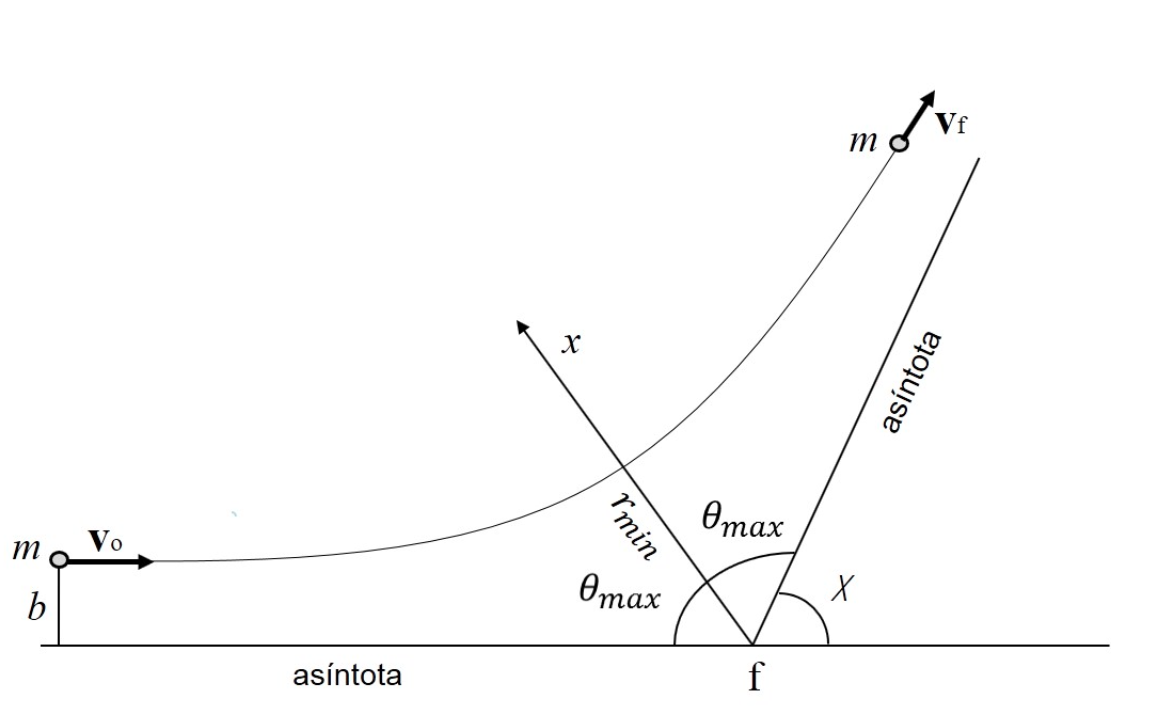
\includegraphics[width=1.8in]{Figuras/Dispersion.png}
   	\end{figure}
	
